%!TEX root = ../lections.tex

Многие биологические объекты обладают периодической структурой. Например, зебра, дождевой червь, сороконожка. Однако известно, что изначально, при появлении, они были однородны. Мы будем рассмотривать случай одномерных структур.

Тьюринг предположил, что существуют два вещества. Одно из них -- $U(x,t)$ -- стимулирует рост клеток. Его назвали активатором. Другое -- $V(x,t)$ -- замедляет рост. Это ингибитор. Следующим предположением было наличие некоторых химических реакций и присутствие диффузии. Фактически, Тьюринг записал уравнение реакции диффузии
\begin{equation}
\left\{\begin{aligned}
	\pdv{U}{t}=f(U,V)+D_1 \pdv[2]{U}{x} \\
	\pdv{V}{t}=g(U,V)+D_2 \pdv[2]{V}{x},
\end{aligned}\right.
	\label{eq:s2:1}
\end{equation}
где $f,g$  - это некоторые нелинейные функции.

Эта система двухкомпонентная, произвольная координата одна. Предположим, \eqref{eq:s2:1} имеет состояние равновесия, т.е. существует решение системы
\begin{equation}
\left\{\begin{aligned}
		f(U,V)=0 \\
		g(U,V)=0
	\end{aligned}\right.	\quad \Rightarrow \quad U=U_0, V=V_0
	\label{eq:s2:2}
\end{equation}
Исследуем уравнение \eqref{eq:s2:1} на устойчивость. Будем подставлять решение, возмущённое около равновесия
\begin{gather*}
	U=U_0+\xi(x,t) \\
	V=V_0+\eta(x,t).
\end{gather*}
Линеаризуем \eqref{eq:s2:1}, подставив туда возмущенное решение, разложив $f, g$ в ряд Тейлора и оставив у них только линейную часть:
\begin{equation}
	\left\{\begin{aligned}
		\pdv{\xi}{t}=f'_u(U_0, V_0)\xi(x,t)+f'_v(U_0, V_0)\eta(x,t)+D_1 \pdv[2]{\xi(x,t)}{x} \\
		\pdv{\eta}{t}=g'_u(U_0, V_0)\xi(x,t)+g'_v(U_0, V_0)\eta(x,t)+D_2 \pdv[2]{\eta(x,t)}{x}.
	\end{aligned}\right.
	\label{eq:s2:3}
\end{equation}

Получили уравнения в частных производных. Будем искать решение в виде
\begin{equation}
	\xi(x,t)=A e^{pt+ikx}, \qquad \eta(x,t)=B e^{pt+ikx}.
	\label{eq:s2:4}
\end{equation}
Сначала перепишем  \eqref{eq:s2:3}, учитывая, что  производные $f'_u(U_0,V_0)$, $f'_v(U_0,V_0)$, а также и $g'_u(U_0,V_0)$, $g'_v(U_0,V_0)$ -- производные в точках (константы) и обозначив их $a$, $b$, $c$, $d$: 
\begin{equation}
	\left\{\begin{aligned}
		&\pdv{\xi}{t}=a\xi+b\eta+D_1 \pdv[2]{\xi}{x} \\
		&\pdv{\eta}{t}=c\xi+d\eta+D_2 \pdv[2]{\eta}{x},
	\end{aligned}\right.
	\label{eq:s2:5}
\end{equation}
Подставляя решение в виде \eqref{eq:s2:4} в \eqref{eq:s2:5}, получим
% где
% \begin{gather*}
% 	a=f'_u(U_0, V_0),~~b=f'_v(U_0, V_0),~~c=g'_u(U_0, V_0),~~d=g'_v(U_0, V_0).
% \end{gather*}
\begin{equation}
	\left\{\begin{aligned}
		&Ap=aA+bB-k^2 D_1A\\
		&Bp=cA+dB-k^2 D_2A,
	\end{aligned}\right.
	\label{eq:s2:6}
\end{equation}

Система \eqref{eq:s2:6} представляет собой систему линейных однородных уравнений относительно констант $A$ и  $B$. Она имеет нетривиальное решение, если ее определитель не равен нулю. Раскрывая определитель, получим характеристическое уравнение для $p$:
\begin{equation}
	p^2+(D_2k^2+D_1k^2-a-d)p+(D_1k^2-a)(D_2k^2-d)-bc=0.
	\label{eq:s2:7}
\end{equation}
Пусть в начальный момент диффузии нет, $D_1=D_2=0$:
\begin{equation}
	p^2-(a+d)p+ad-bc=0.
	\label{eq:s2:8}
\end{equation}
\begin{figure}[H]
	\centering
	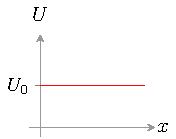
\includegraphics[scale=1.5]{img/diffusion_instability/static_u} 
	\caption{Устойчивая в отсутствии диффузии система}
\end{figure}
Предположим, что без диффузии система устойчива ($\Re p < 0$). Условие для этого
\begin{gather}
	\Delta_0=ad-bc>0, \qquad \sigma_0=a+d<0,
	\label{eq:s2:9}
\end{gather}
В этом (устойчивом) случае по оси $x$ активатор $U$ и ингибитор $V$ постоянны. 

Пусть теперь $D_1, D_2 \neq 0$. В этом случае \eqref{eq:s2:7} после преобразований примет вид:
\begin{gather*}
	p^2-\sigma p+\Delta=0, \quad \text{где}\\
	\Delta=a+d-(D_1+D_2)k^2=\sigma_0-(D_1+D_2)k^2, \\ \sigma=ad-bc-(aD_2+dD_1)k^2+D_1D_2k^4=\Delta_0-(aD_2+dD_1)k^2+D_1D_2k^4.
\end{gather*}
Несложный анализ показывает следующую зависимость $\Re p$  от $k^2$:
\begin{figure}[h]
\begin{minipage}[h]{0.49\linewidth}
\center{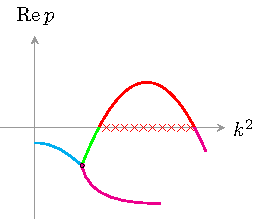
\includegraphics[scale=1.5]{img/diffusion_instability/re_p}}
\end{minipage}
\hfill
\begin{minipage}[h]{0.49\linewidth}
\center{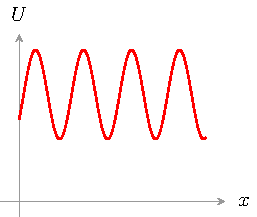
\includegraphics[scale=1.5]{img/diffusion_instability/u_x}}
\end{minipage}
	\caption{Зависимость $\Re p$ от $k^2$ при $D_{1,2}\ne0$ и структура Тьюринга (справа)}
\end{figure}

Есть диапазон, где произошла потеря устойчивости состояния равновесия за счет действия диффузии. Такую потерю устойчивости называют \textbf{диффузионной неустойчивостью}.При этом оказывается, что возникает аналог бифуркации Андронова-Хопфа. 

Возникает периодическое по пространству (в нашем случае -- по $x$) решение, и это решение пространственно-неоднородное и переодическое (структура, паттерн). Оказыватся, этот паттерн структурно устойчив.

Динамическая структура, обладающая свойством структурной устойчивости, иногда называется диссипативной структурой. Она возникает за счет баланса активатора и ингибитора. 

После открытия Тьюрингом возможности существования таких паттернов за счет активатора и ингибитора, были реально обнаружены в природе такие вещества.



\subsection{Простые волны. Образование разрывов.}
Рассмотрим однородную линейную среду без дисперсии, свойства которой описывает скалярная функция $U(x,t)$. В таких средах возможны волновые движения, при этом все переменные описываются одинаковыми уравнениями
\begin{equation}
	\pdv{U_j}{t}+V\pdv{U_j}{x}=0,
	\label{eq:s2:10}
\end{equation}
где $V$ -- константа. В среде нет собственных масштабов и нелинейностей. В этой среде возможно существование так называемых римановых волн
\begin{equation}
	U_j=\phi(x-Vt),
	\label{eq:s2:11}
\end{equation}
где $\phi$ - произвольная, обязательно дифференцируемая, функция.

Проверим прямой подстановкой. Введем бегущую координату $\xi=x-Vt$ и подставим \eqref{eq:s2:11} в \eqref{eq:s2:10}:
\begin{gather*}
	\dv{\phi}{\xi} \pdv{\xi}{t}+V\dv{\phi}{\xi} \pdv{\xi}{x}=0
	\quad\Rightarrow\quad
	-V\dv{\phi}{\xi}+V \dv{\phi}{\xi} \equiv 0.
\end{gather*}
Значит, \eqref{eq:s2:11} действительно является решением такой системы. 

Теперь рассмотрим нелинейную среду без дисперсии. Оказывается, в таких средах могут существовать волны, которые сохраняют одно свойство римановых:  переменные связаны алгебраически (если есть $U_1$ и $U_2$, то $U_3$ всегда можно пересчитать). 



\newpage
\paragraph{Волны на мелкой воде. } Типичный пример таких волн -- волны на мелкой воде, $\lambda \gg h_0$ (см. рис. ниже). Это гравитационные волны, бегущие вдоль оси $x$. 
Состояние жидкости описывается скоростью волны $V$  и профилем $h(z)$. Поскольку волны длинные, считаем, что $V$ не зависит от $z$.

\begin{figure}[H]
	\centering
	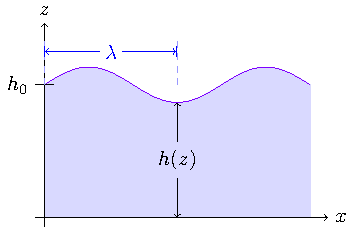
\includegraphics[scale=1.5]{img/diffusion_instability/long_waves}
\end{figure}

Запишем уравнение Эйлера. Жидкость несжимаемая ($\rho=\const$): 
\begin{gather*}
	\pdv{V}{t}+V\pdv{V}{x}+\frac1{\rho}\pdv{p}{x}=0
	% , \\ \rho=const, p-\text{среднее по высоте}, \\ \.
\end{gather*}
Давление больше там, где выше жидкость: $\frac1{\rho}\pdv{p}{x}=g\pdv{h}{x}$, тогда
\begin{equation}
	\pdv{V}{t}+V\pdv{V}{x}+g\pdv{h}{x}=0.
	\label{eq:s2:12}
\end{equation}
Второе уравнение -- уравнение непрерывности (в терминах потоков через близкие сечения скорость изменения высоты слоя связана с разностью потока через $x$ и $\dd x$):
\begin{equation}
	\pdv{h}{t}+\pdv{(Vh)}{x}=0. 
	\quad \Rightarrow \quad
	\pdv{h}{t}+V\pdv{h}{x}+h\pdv{V}{x}=0.
	\label{eq:s2:13}
\end{equation}

Предположим, что $h$ и $V$ не являются независимыми переменными и $h=h(V)$, тогда $\pdv{h}{x}=\dv{h}{V}\pdv{V}{x}$ и из уравнения \eqref{eq:s2:12} будет следовать, что 
\begin{gather*}
	\pdv{V}{t}+V\pdv{V}{x}+g\pdv{h}{x} = 0.
	 % ~(*)
	 \tag{*}
\end{gather*}
Аналогично подставим в уравнение \eqref{eq:s2:13}, тогда
\begin{gather*}
	\dv{h}{V}\pdv{V}{t}+V\dv{h}{V}\pdv{V}{x}+h(V)\pdv{V}{x} = 0
	\quad \Rightarrow \quad
	\pdv{V}{t}+V\pdv{V}{x}+\frac{h(V)}{\dv{h}{V}}\pdv{h}{x} = 0.
	\tag{**}
\end{gather*}
Уравнения (*) и (**) должны совпадать, так как описывают одну и ту же величину. Значит, нужно прировнять коэффициенты при производных, и тогда получим уравнение для нахождения $h$:
\begin{equation*}
	g\dv{h}{V}=\frac{h}{\dv{h}{V}}
	\quad \Rightarrow \quad
	\dv{h}{V}=\pm \sqrt{\frac{h(V)}{g}}
\end{equation*}
Подставив полученное выражение в (**), получим уравнение простой волны
\begin{equation}
	\pdv{V}{t}+V\pdv{V}{x}\pm \sqrt{h(V)g\,} \pdv{V}{x} = 0
	\quad \Rightarrow \quad
	\pdv{V}{t}+\qty(V\pm \sqrt{h(V)g}\,)\pdv{V}{x} = 0.
	\label{eq:s2:14}
\end{equation}

\paragraph{Уравнение простой волны. } В общем виде это уравнение справедливо не только на мелкой воде, и выглядит следующим образом:
\begin{equation}
	\pdv{U}{t}+V(U)\pdv{U}{x} = 0
	\label{eq:s2:15}
\end{equation}
Здесь $V$ -- это функция среды. 

Давайте исследуем уравнение \eqref{eq:s2:15}. Будем искать решение в виде
\begin{equation}
	U = \phi(\xi), \quad \text{где}\quad
	\xi=x-V(U)t.
	\label{eq:s2:16}
\end{equation}
Убедимся, что \eqref{eq:s2:16} - решение. Найдём производные в силу \eqref{eq:s2:16}:
\begin{gather}
	\nonumber\pdv{U}{t}=\dv{\phi}{\xi}\pdv{\xi}{t}=\dv{\phi}{\xi}\qty(-V(U)-t\dv{V}{U}\pdv{U}{t})
	\,\Rightarrow \\ \Rightarrow 
	\pdv{U}{t}\qty(1+\dv{\phi}{\xi}\dv{V}{U}t)=-V(U)\dv{\phi}{\xi}
	\vspace{-0.5em}\quad \Rightarrow \vspace{-0.5em}\quad
	\pdv{U}{t}=-V(U)\frac{\dv{\phi}{\xi}}{\qty(1+\dv{\phi}{\xi}\dv{V}{U}t)}
	\label{eq:s2:6}
\end{gather}
Аналогичным образом получается
\begin{gather*}
	\pdv{U}{x}=\dv{\phi}{\xi} \frac{1}{\qty(1+\dv{\phi}{\xi}\dv{V}{U}t)}.
\end{gather*}
Действительно, подставляя полученные выражения в \eqref{eq:s2:15}, получим тождество.

Исследуем решение \eqref{eq:s2:16}. Для определенности зададим вид нелинейности $V(U)$ и профиль волны в начальный момент времени $\phi(x,t=0)$\footnote{Есть два способа исследования: задать начальное распределение по $x$ и смотреть, что с ним будет происходить во времени, или наоборот -- создать на границе постоянные колебания и смотреть, что с ними произойдет при распространении вдоль $x$} (см. рис. \ref{fig:uvux}).

\begin{figure}[H]
\begin{minipage}[h]{0.49\linewidth}
\center{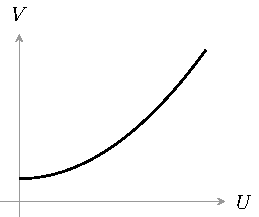
\includegraphics[scale=1.4]{img/diffusion_instability/vu}}
\end{minipage}
\hfill
\begin{minipage}[h]{0.49\linewidth}
\center{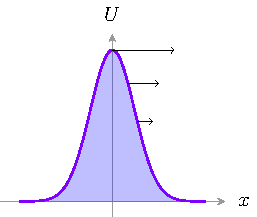
\includegraphics[scale=1.4]{img/diffusion_instability/ux}}
\end{minipage}
	\caption{}
	\label{fig:uvux}
\end{figure}

% У максимального значения U скорость наибольшая. Задается профиль $\phi$ при $t=0$:
% \begin{figure}[H]
% 	\centering
% 	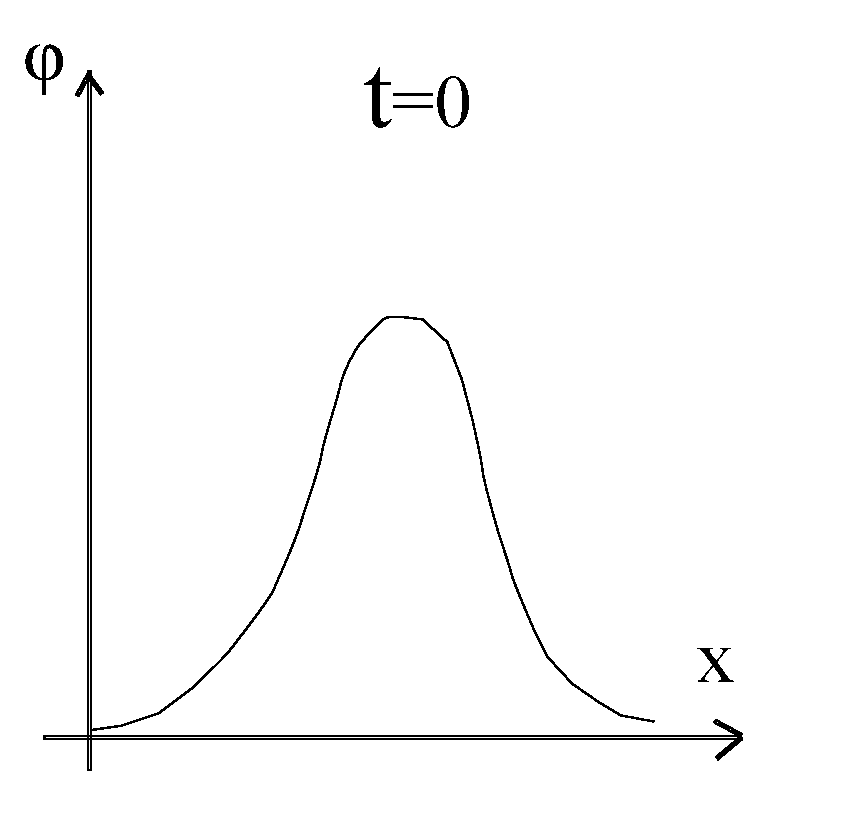
\includegraphics[width=0.4\linewidth]{fig/fig13.pdf}   
% \end{figure}
% или при $x=0$:
% \begin{figure}[H]
% 	\centering
% 	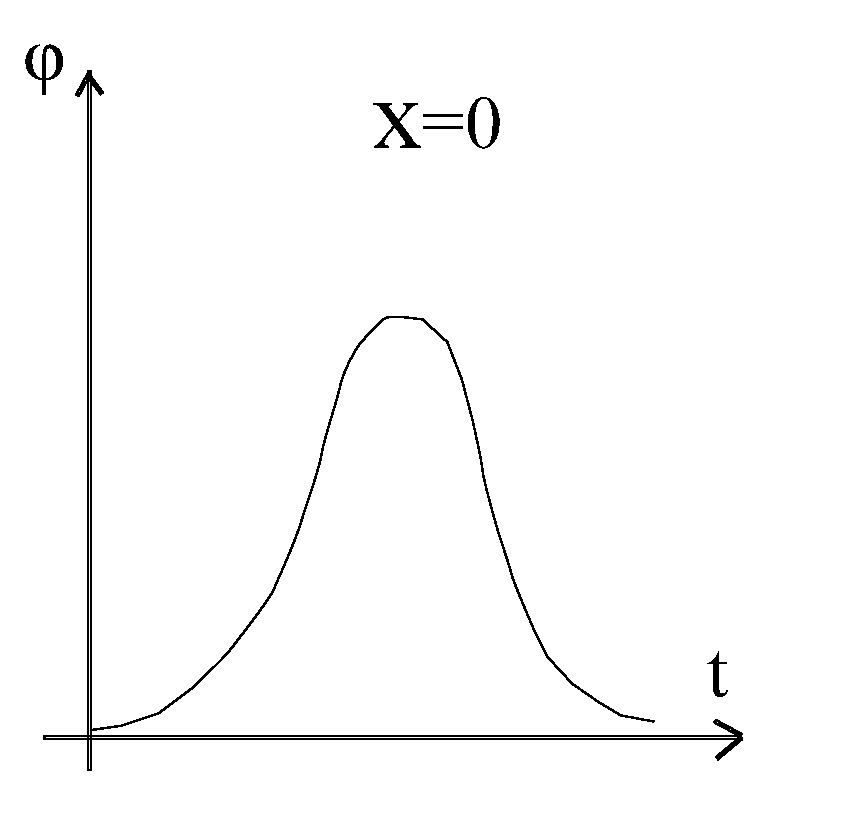
\includegraphics[width=0.4\linewidth]{fig/fig14.pdf}   
% \end{figure}
Во время распространения гребень волны будет обгонять подошву волны, будет просходить укручение фронта: волна деформируется.
\begin{figure}[H]
	\centering
	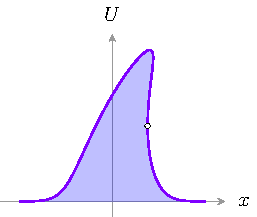
\includegraphics[scale=1.4]{img/diffusion_instability/ux2.pdf}
\end{figure}
% \begin{figure}[H]
% 	\centering
% 	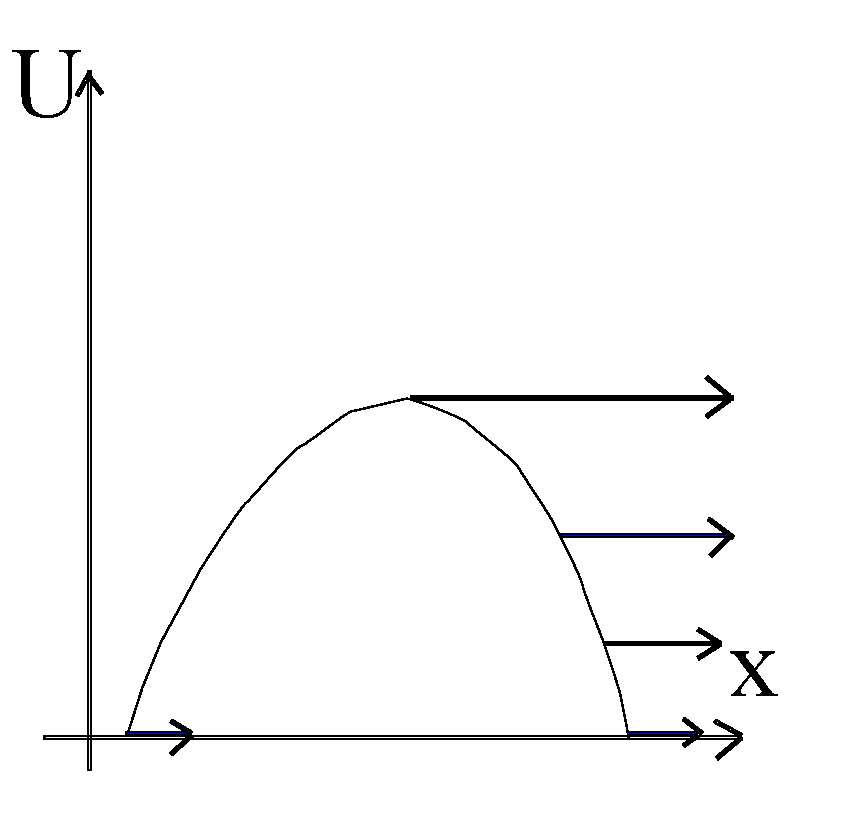
\includegraphics[width=0.4\linewidth]{fig/fig15.pdf}   
% \end{figure}
% \begin{figure}[H]
% 	\centering
% 	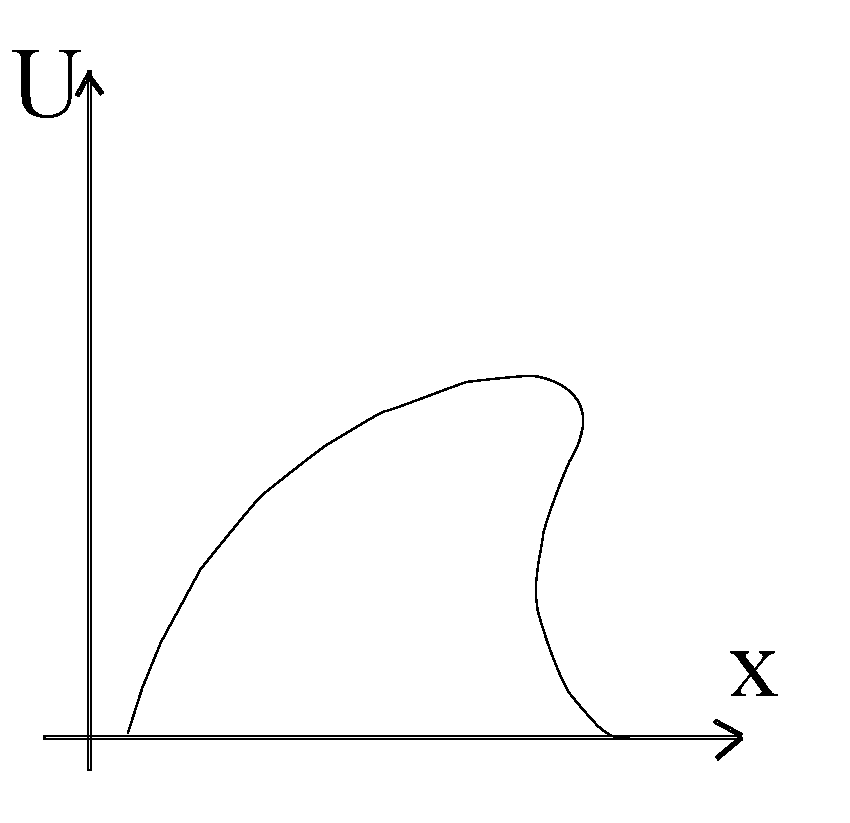
\includegraphics[width=0.4\linewidth]{fig/fig16.pdf}   
% \end{figure}
% \begin{figure}[H]
% 	\centering
% 	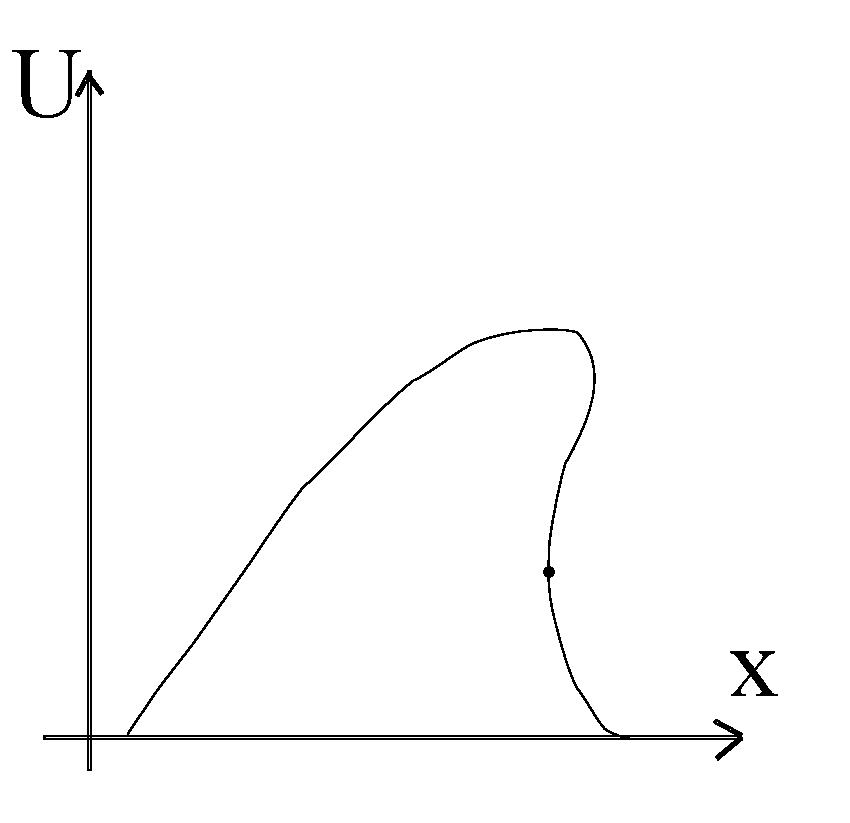
\includegraphics[width=0.4\linewidth]{fig/fig17.pdf}   
% \end{figure}
В момент времени
\begin{equation}
	1+\dv{\phi}{\xi}\dv{V}{U} t = 0
\end{equation}
появится точка, где производные $\pdv{U}{t}, \pdv{U}{x} \rightarrow \infty $. Образуется бесконечный градиент и разрыв, который характеризуется состоянием $U^*, t^*, x^*$. Дальнейшее описание в рамках простой волны невозможно. Такой момент в решении называют \textbf{градиентной катастрофой}. %Вторые производные тоже обращаются в бесконечность, и точки эти можно найти.